\documentclass[12pt,letter]{article}
\usepackage[moduleName={Super Echo}]{KautenjaDSP}
\begin{document}
\titlePage{img/Logo}{img/Module}{img/KautenjaDSP}

% -------------------
% MARK: Overview
% -------------------

\section{Overview}

Super Echo is a Eurorack module that emulates the echo effect from the S-SMP sound chip on the Super Nintendo Entertainment System (SNES). The Echo effect of the S-SMP chip has $15$ different delay levels of $16ms$ each, a $64KB$ echo buffer, an 8-tap FIR filter for shaping the sound of the echo, parameterized feedback, and parameterized dry / wet mix level. The echo buffer is stereo, although the echo parameters and coefficients of the FIR filter are the same for both channels. Super Echo provides the key features of the echo module of the S-SMP chip, namely,
\begin{itemize}
  \item \textbf{Stereo Processing:} Dual echo buffers for two independent inputs in stereo configuration.
  \item \textbf{Expanded Delay:} The 15 levels of delay has been upgraded to 31 levels that each add an additional $16ms$ of delay (up to roughly $500ms$).
  \item \textbf{Feedback:} Additive and subtractive feedback following the original implementation
  \item \textbf{8-tap FIR Filter:} Fully parameterized 8-tap FIR filter for shaping the sound of the echo. The filter can be parameterized as low-pass, high-pass, band-pass, band-stop, etc. and includes presets with filter parameters from popular SNES games.
\end{itemize}

\begin{figure}[!b]
\centering
\includegraphics[width=0.5\textwidth]{img/Chip}
\caption*{\small The S-SMP module from the SNES. The S-SMP included two discrete microprocessors: the SPC700, and the S-DSP. The SPC700 performed primary computation, while the S-DSP performed DSP specific computations, like BRR decoding, sample playback, applying the echo effect, mixing levels, etc. The SPC700 and S-DSP shared $64KB$ of total RAM that was used for BRR sample data and the echo buffer. The digital audio is decoded back to an analog signal by a 16-bit DAC and amplified using an Op-Amp. Before digital-to-analog conversion, the output audio is low-pass filtered by a Gaussian filter that gives the S-SMP chip a distinctive sound.}
\end{figure}

% -------------------
% MARK: Panel Layout
% -------------------

\clearpage
\section{Panel Layout}

\begin{figure}[!htp]
\centering
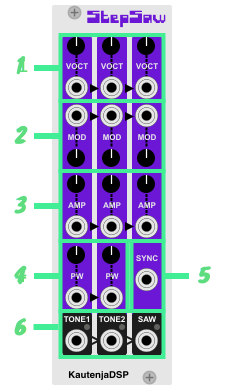
\includegraphics{img/Interface}
\end{figure}

\subsection{Audio Input}

The module accepts both mono and stereo inputs. If an input is patched to the left \textbf{IN} port, but not the right \textbf{IN} port, the signal is normalled from the left input to the right input. The \textbf{IN} trimpot acts as a gain control for the individual processing lanes in the range of $[-\infty, 6]dB$. VU meter lights measure the input of individual processing lanes going from off ($-\infty dB$ to $-12dB$), to green ($-12dB$ to $0dB$), and lastly to red ($0dB$ to $6dB$) when clipping begins to occur. Input voltages are clipped to $10V_{pp}$ (i.e., $[-5, 5]V$) for digital processing in the S-SMP emulation. When using Super VCA for audio rate signals in the standard $10V_{pp}$ range, $0dB$ gain will fully saturate the signal\footnote{Some oscillators produce band-limited signals that are mostly $10V_{pp}$, but may have some time-domain ripples outside this range that will be clipped. This will introduce aliasing.}. If using the module to attenuate control voltages in the range of $[-10, 10]V$, a gain setting of at most $-6dB$ is optimal to prevent clipping the signal.

\subsection{Mix Level}

When no input is connected, the \textbf{MIX} trimpot controls the mix level with 8-bit signed resolution (i.e., $\in [-128, 127]$). Negative volumes will invert the phase of the mixed echo signal, and can be used for interesting surround sound effects when modulated independently between the stereo pair. When the mix is 0, the output from the module is the purely dry signal. When mix is fully clockwise, the echo is fully mixed into the dry signal on output. When the mix is fully counter-clockwise, the inverted echo signal is fully mixed into the dry signal on output. When an input is patched to the \textbf{MIX} port, the \textbf{MIX} trimpot acts like an attenuverter that polarizes and scales the CV control over the mix level. Inputs are normalled from the left input to the right input.

\subsection{Delay and Feedback}

The \textbf{DELAY} trimpot controls the delay level in increments of $16ms$ (at $f_s = 32kHz$). The original S-SMP chip was limited to 15 levels of delay due to the $64kB$ RAM on the chip that had to be shared with sample data. Super Echo extends the size of the RAM buffer to the full $64kB$ bank, meaning there are now 31 delay levels, with maximal delays of $512ms$. When an input is patched to the \textbf{DELAY} port, the \textbf{DELAY} trimpot sets the base delay level, and the CV controls the offset in increments of $\approx250mV$.

The \textbf{FEEDBACK} trimpot controls the amount of feedback in the echo buffer with 8-bit signed resolution (i.e., $\in [-128, 127]$). Negative values will invert the phase of the echo signal feedback. When an input is patched to the \textbf{FEEDBACK} port, the \textbf{FEEDBACK} trimpot sets the base feedback level, and the CV controls the offset.

\subsection{FIR Filter Coefficients}

The echo effect of the S-SMP featured a programmable multi-mode filter that could be configured as low-pass, high-pass, band-pass, or band-stop to shape the color of the feedback in the echo buffer\footnote{The \textbf{FEEDBACK} parameter must have a \textit{magnitude} greater than $0$ for the FIR filter to have an effect on the signal.}. The filter was implemented as an 8-tap finite impulse response (FIR) filter with signed 8-bit coefficients (i.e., $\in [-128, 127]$) that could be programmed into the game music. Super Echo exposes these FIR coefficients with slider and CV controls. The \textbf{FIR} sliders set the value of the coefficient where the center position is $0$, left of center produces negative values down to $-128$, and right of center produces positive values up to $127$. When an input is patched to a port, the slider controls the base value and the CV controls the offset. The \textbf{FIR} trimpots can be used to attenuate and polarize the individual CVs for each coefficient. The \textbf{FIR} input ports are normalled in a chain that can be broken to quickly control all the FIR coefficients with only a few modulation sources and patch cables using the individual CV attenuverters.

\subsection{Audio Output}

Each processing lane produces an output signal of at most $10V_{pp}$ (i.e., $[-5, 5]V$) on the \textbf{OUT} port. VU meter lights measure the output of individual channels going from off ($-\infty dB$ to $-12dB$), to green ($-12dB$ to $0dB$), and lastly to red ($0dB$ to $6dB$) when clipping begins to occur due to excessive feedback.

\subsection{Bypass}

The \textbf{BYPASS} switch allows the circumvention of the S-SMP Gaussian interpolation filter emulation without breaking the stereo signal path. When the bypass switch is pointing up, the input signals only pass through the gain circuit before passing to their respective outputs. When the bypass switch is pointing down, the gained inputs pass through the S-SMP Gaussian interpolation filter emulation.

\end{document}
